\documentclass[11pt,a4paper]{article}
\usepackage{lmodern}

\usepackage{amssymb,amsmath}
\usepackage{ifxetex,ifluatex}
\usepackage{fixltx2e} % provides \textsubscript
\ifnum 0\ifxetex 1\fi\ifluatex 1\fi=0 % if pdftex
  \usepackage[T1]{fontenc}
  \usepackage[utf8]{inputenc}
\else % if luatex or xelatex
  \ifxetex
    \usepackage{mathspec}
    \usepackage{xltxtra,xunicode}
  \else
    \usepackage{fontspec}
  \fi
  \defaultfontfeatures{Mapping=tex-text,Scale=MatchLowercase}
  \newcommand{\euro}{???}
\fi
% use upquote if available, for straight quotes in verbatim environments
\IfFileExists{upquote.sty}{\usepackage{upquote}}{}
% use microtype if available
\IfFileExists{microtype.sty}{%
\usepackage{microtype}
\UseMicrotypeSet[protrusion]{basicmath} % disable protrusion for tt fonts
}{}
\usepackage[lmargin=2.5cm,rmargin=2.5cm,tmargin=2.5cm,bmargin=2.5cm]{geometry}

% Figure Placement:
\usepackage{float}
\let\origfigure\figure
\let\endorigfigure\endfigure
\renewenvironment{figure}[1][2] {
    \expandafter\origfigure\expandafter[H]
} {
    \endorigfigure
}

%% citation setup
\usepackage{csquotes}

\usepackage[backend=biber, maxbibnames = 99, style = apa]{biblatex}
\setlength\bibitemsep{1.5\itemsep}
\addbibresource{R_packages.bib}
\bibliography{references.bib}
\usepackage{color}
\usepackage{fancyvrb}
\newcommand{\VerbBar}{|}
\newcommand{\VERB}{\Verb[commandchars=\\\{\}]}
\DefineVerbatimEnvironment{Highlighting}{Verbatim}{commandchars=\\\{\}}
% Add ',fontsize=\small' for more characters per line
\usepackage{framed}
\definecolor{shadecolor}{RGB}{248,248,248}
\newenvironment{Shaded}{\begin{snugshade}}{\end{snugshade}}
\newcommand{\AlertTok}[1]{\textcolor[rgb]{0.94,0.16,0.16}{#1}}
\newcommand{\AnnotationTok}[1]{\textcolor[rgb]{0.56,0.35,0.01}{\textbf{\textit{#1}}}}
\newcommand{\AttributeTok}[1]{\textcolor[rgb]{0.77,0.63,0.00}{#1}}
\newcommand{\BaseNTok}[1]{\textcolor[rgb]{0.00,0.00,0.81}{#1}}
\newcommand{\BuiltInTok}[1]{#1}
\newcommand{\CharTok}[1]{\textcolor[rgb]{0.31,0.60,0.02}{#1}}
\newcommand{\CommentTok}[1]{\textcolor[rgb]{0.56,0.35,0.01}{\textit{#1}}}
\newcommand{\CommentVarTok}[1]{\textcolor[rgb]{0.56,0.35,0.01}{\textbf{\textit{#1}}}}
\newcommand{\ConstantTok}[1]{\textcolor[rgb]{0.00,0.00,0.00}{#1}}
\newcommand{\ControlFlowTok}[1]{\textcolor[rgb]{0.13,0.29,0.53}{\textbf{#1}}}
\newcommand{\DataTypeTok}[1]{\textcolor[rgb]{0.13,0.29,0.53}{#1}}
\newcommand{\DecValTok}[1]{\textcolor[rgb]{0.00,0.00,0.81}{#1}}
\newcommand{\DocumentationTok}[1]{\textcolor[rgb]{0.56,0.35,0.01}{\textbf{\textit{#1}}}}
\newcommand{\ErrorTok}[1]{\textcolor[rgb]{0.64,0.00,0.00}{\textbf{#1}}}
\newcommand{\ExtensionTok}[1]{#1}
\newcommand{\FloatTok}[1]{\textcolor[rgb]{0.00,0.00,0.81}{#1}}
\newcommand{\FunctionTok}[1]{\textcolor[rgb]{0.00,0.00,0.00}{#1}}
\newcommand{\ImportTok}[1]{#1}
\newcommand{\InformationTok}[1]{\textcolor[rgb]{0.56,0.35,0.01}{\textbf{\textit{#1}}}}
\newcommand{\KeywordTok}[1]{\textcolor[rgb]{0.13,0.29,0.53}{\textbf{#1}}}
\newcommand{\NormalTok}[1]{#1}
\newcommand{\OperatorTok}[1]{\textcolor[rgb]{0.81,0.36,0.00}{\textbf{#1}}}
\newcommand{\OtherTok}[1]{\textcolor[rgb]{0.56,0.35,0.01}{#1}}
\newcommand{\PreprocessorTok}[1]{\textcolor[rgb]{0.56,0.35,0.01}{\textit{#1}}}
\newcommand{\RegionMarkerTok}[1]{#1}
\newcommand{\SpecialCharTok}[1]{\textcolor[rgb]{0.00,0.00,0.00}{#1}}
\newcommand{\SpecialStringTok}[1]{\textcolor[rgb]{0.31,0.60,0.02}{#1}}
\newcommand{\StringTok}[1]{\textcolor[rgb]{0.31,0.60,0.02}{#1}}
\newcommand{\VariableTok}[1]{\textcolor[rgb]{0.00,0.00,0.00}{#1}}
\newcommand{\VerbatimStringTok}[1]{\textcolor[rgb]{0.31,0.60,0.02}{#1}}
\newcommand{\WarningTok}[1]{\textcolor[rgb]{0.56,0.35,0.01}{\textbf{\textit{#1}}}}
\usepackage{longtable,booktabs}
\usepackage{graphicx}
\makeatletter
\def\maxwidth{\ifdim\Gin@nat@width>\linewidth\linewidth\else\Gin@nat@width\fi}
\def\maxheight{\ifdim\Gin@nat@height>\textheight\textheight\else\Gin@nat@height\fi}
\makeatother
% Scale images if necessary, so that they will not overflow the page
% margins by default, and it is still possible to overwrite the defaults
% using explicit options in \includegraphics[width, height, ...]{}
\setkeys{Gin}{width=\maxwidth,height=\maxheight,keepaspectratio}
\ifxetex
  \usepackage[setpagesize=false, % page size defined by xetex
              unicode=false, % unicode breaks when used with xetex
              xetex]{hyperref}
\else
  \usepackage[unicode=true, linktocpage = TRUE]{hyperref}
\fi
\hypersetup{breaklinks=true,
            bookmarks=true,
            pdfauthor={Author 1, Author 2, Author 3},
            pdftitle={The Title of Your Seminar Paper},
            colorlinks=true,
            citecolor=blue,
            urlcolor=blue,
            linkcolor=magenta,
            pdfborder={0 0 0}}
\urlstyle{same}  % don't use monospace font for urls
\setlength{\parindent}{0pt}
\setlength{\parskip}{6pt plus 2pt minus 1pt}
\setlength{\emergencystretch}{3em}  % prevent overfull lines
\setcounter{secnumdepth}{5}

%%% Use protect on footnotes to avoid problems with footnotes in titles
\let\rmarkdownfootnote\footnote%
\def\footnote{\protect\rmarkdownfootnote}

%%% Change title format to be more compact
\usepackage{titling}

% Create subtitle command for use in maketitle
\newcommand{\subtitle}[1]{
  \posttitle{
    \begin{center}\large#1\end{center}
    }
}

\setlength{\droptitle}{-2em}
  \title{The Title of Your Seminar Paper}
  \pretitle{\vspace{\droptitle}\centering\huge}
  \posttitle{\par}
\subtitle{Course}
  \author{Author 1, Author 2, Author 3}
  \preauthor{\centering\large\emph}
  \postauthor{\par}
  \predate{\centering\large\emph}
  \postdate{\par}
  \date{today}


%% linespread settings

\usepackage{setspace}

\onehalfspacing

% Language Setup

\usepackage{ifthen}
\usepackage{iflang}
\usepackage[super]{nth}
\usepackage[ngerman, english]{babel}

%Acronyms
\usepackage[printonlyused, withpage, nohyperlinks]{acronym}
\usepackage{changepage}

% Multicols for the Title page
\usepackage{multicol}


\usepackage{longtable}

\begin{document}

\selectlanguage{english}


%\maketitle

\begin{titlepage}
  \noindent\begin{minipage}{0.6\textwidth}
	  \IfLanguageName{english}{University of Duisburg-Essen}{Universit\"at Duisburg-Essen}\\
	  \IfLanguageName{english}{Faculty of Business Administration and Economics}{Fakult\"at f\"ur Wirtschaftswissensschaften}\\
	  \IfLanguageName{english}{Chair of Econometrics}{Lehrstuhl f\"ur \"Okonometrie}\\
  \end{minipage}
	\begin{minipage}{0.4\textwidth}
	  \begin{flushright}
  	  \vspace{-0.5cm}
      \IfLanguageName{english}{\includegraphics*[width=5cm]{Includes/duelogo_en.png}}{\includegraphics*[width=5cm]{Includes/duelogo_de.png}}
	  \end{flushright}
	\end{minipage}
  \\
  \vspace{1.5cm}
  \begin{center}
  \huge{The Title of Your Seminar Paper}\\
  \vspace{.25cm}
  \Large{Course}\\
  \vspace{0.5cm}
  \large{Term Paper}\\
  \vspace{1cm}
  \large{
  \IfLanguageName{english}{Submitted to the Faculty of \\ Business Administration and Economics \\at the \\University of Duisburg-Essen}{Vorgelegt der \\Fakult\"at f\"ur Wirtschaftswissenschaften der \\ Universit\"at Duisburg-Essen}\\}
  \vspace{0.75cm}
  \large{\IfLanguageName{english}{from:}{von:}}\\
  \vspace{0.5cm}
  Author 1, Author 2, Author 3\\
  \end{center}
  %\vspace{2cm}
  \vfill
  \hrulefill

  \noindent\begin{minipage}[t]{0.3\textwidth}
  \IfLanguageName{english}{Reviewer:}{Erstgutachter:}
  \end{minipage}
  \begin{minipage}[t]{0.7\textwidth}
  \hspace{1cm}(Prof.) Dr.~XYZ
  \end{minipage}

  \noindent\begin{minipage}[t]{0.3\textwidth}
  \IfLanguageName{english}{Deadline:}{Abgabefrist:}
  \end{minipage}
  \begin{minipage}[t]{0.7\textwidth}
  \hspace{1cm}tomorrow
  \end{minipage}

  \hrulefill

  \begin{multicols}{4}

  Name:

  Matriculation No.:

  E-Mail:

  Study Path:

  Semester:

  Graduation (est.):

  \columnbreak

  Ape Monkey

  123456

  Ape@Monkey.biz

  M.Sc. Economics

  \nth{5}

  Summer Term 2020

  \columnbreak

  John Doe

  234567

  john.doe@web.de

  M.Sc. Economics

  \nth{4}

  Summer Term 2020

  \columnbreak

  Darth Vader

  543556

  vader@emperialenterprises.com

  M.Sc. Economics

  \nth{3}

  Summer Term 2020

  \end{multicols}

\end{titlepage}

\newgeometry{top=2cm, left = 5cm, right = 2.5cm, bottom = 2.5cm}


\pagenumbering{Roman}
{
\hypersetup{linkcolor=black}

\setcounter{tocdepth}{3}
\tableofcontents
}

\newpage
\listoffigures
\addcontentsline{toc}{section}{List of Figures}

%\newpage
\listoftables
\addcontentsline{toc}{section}{List of Tables}

\section*{List of Abbreviations}
\addcontentsline{toc}{section}{List of Abbreviations}

\begin{adjustwidth}{1.5em}{0pt}

\begin{acronym}[dummyyyy]
 \acro{ECTSCP}{European Credit Transfer System Credit Point}
 \acro{lasso}{Least Absolute Shrinkage and Selection Operator}
 \acro{pcr}{Principal Components Regression}
 \acro{pls}{Partial Least Squares}
 \acro{RMSE}{Root Mean Squared Error}
 \acroplural{LRG}[LRG]{laengefristige Refinanzierungsgeschaefte}

%Falls eine Abkuerzung in der Mehrzahl nicht einfach auf "s" endet muss das speziell eingestellt werden.
% \acro{slmtA}{super lange mega tolle Abkuerzung} %Einzahl
 %\acroplural{slmtA}[slmtAs]{super lange mega tolle Abkuerzungen} %Mehrzahl
 \acro{dummyyyy}{dummyyy}
\end{acronym}

\end{adjustwidth}

\restoregeometry

\newpage
\pagenumbering{arabic}
\hypertarget{rmarkdown-template}{%
\section{Rmarkdown Template}\label{rmarkdown-template}}

Currently there is one thing you need to customise manually in
\emph{template.tex} which will be used by the \LaTeX processor for
generating the PDF: the entries in the columns on the title page
containing student info. Here you have to replace the dummy data:

\begin{verbatim}
\begin{multicols}{$cols_authors$}

Name:

Matriculation No.:

E-Mail:

Study Path:

Semester:

Graduation (est.):
\end{verbatim}

If you are just two people, working alone or want to remove the colum
design you may delete (parts of) this section.

\hypertarget{r-markdown}{%
\subsection{R Markdown}\label{r-markdown}}

This is an R Markdown document. Markdown is a simple formatting syntax
for authoring HTML, PDF, and MS Word documents. For more details see
\url{http://rmarkdown.rstudio.com}.

You may use \LaTeX~to write formulas, e.g., \(X^2 = \sqrt{X^4}\) and
\[X^2 = \sqrt{X^4}.\]

After clicking the \emph{Knit} button in \emph{RStudio}, a (PDF)
document that includes both content and the output of any embedded R
code chunks will be generated.

You can embed an R code chunk like this:

\begin{Shaded}
\begin{Highlighting}[]
\KeywordTok{summary}\NormalTok{(cars)}
\end{Highlighting}
\end{Shaded}

\begin{verbatim}
##      speed           dist       
##  Min.   : 4.0   Min.   :  2.00  
##  1st Qu.:12.0   1st Qu.: 26.00  
##  Median :15.0   Median : 36.00  
##  Mean   :15.4   Mean   : 42.98  
##  3rd Qu.:19.0   3rd Qu.: 56.00  
##  Max.   :25.0   Max.   :120.00
\end{verbatim}

\hypertarget{including-plots}{%
\subsection{Including Plots}\label{including-plots}}

You can also embed plots, for example:

\begin{figure}
\centering
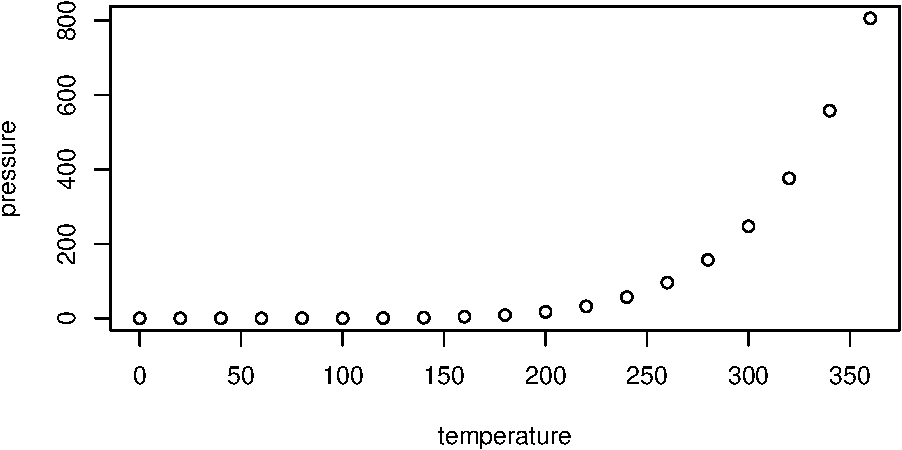
\includegraphics{Seminararbeit_files/figure-latex/pressure-1.pdf}
\caption{\label{fig:pressure} Pressure}
\end{figure}

Note that the \texttt{echo\ =\ FALSE} parameter was added to the code
chunk to prevent printing of the R code that generated the plot. You can
label the plot above by including the label
\texttt{\textbackslash{}\textbackslash{}label\{fig:pressure\}} in the
chunk argument \texttt{fig.cap}. A reference to the plot is then made as
follows:

Looking at Figure \ref{fig:pressure} makes me happy.

\hypertarget{the-yaml-header}{%
\subsection{The YAML Header}\label{the-yaml-header}}

The YAML header is at the very top of this document. It is enclosed by 3
dashes. Although some useful options are specified already (most of
which are hopefully self-explaining) you may want additional
customisation. Below we discuss useful options that we have implemented
for you.

\emph{Note that \textbf{indentation and line breaks matter} in the YAML
header.} More about that
\href{https://learn-the-web.algonquindesign.ca/topics/markdown-yaml-cheat-sheet/\#yaml}{here}.

\hypertarget{language}{%
\subsubsection{\texorpdfstring{\texttt{language}}{language}}\label{language}}

This variable affects mainly the headings of your output file and
automatic hyphenation.

You can set this to \texttt{english} or \texttt{german} like this:

\texttt{language:\ english}

\texttt{language:\ german}

If the language is not specified in the YAML header it will be set to
\texttt{english}.

\hypertarget{linespread}{%
\subsubsection{\texorpdfstring{\texttt{linespread}}{linespread}}\label{linespread}}

The default value for the linespread is 1.5. Usually this is fine and
sometimes it's required. If you nevertheless want to change it you can
do so by specifying the linespread variable, e.g.

\texttt{linespread:\ 1}

\hypertarget{rmarkdown-makes-your-life-easy}{%
\section{Rmarkdown makes your life
easy}\label{rmarkdown-makes-your-life-easy}}

\hypertarget{the-kable-function}{%
\subsection{The kable function}\label{the-kable-function}}

In empirical work it's crucial not only to present your results but also
to explain your research strategy. This often involves tables presenting
data and results. Generating tables by hand using \LaTeX is an option
but may be time consuming. However, there is a variety of R packages
that automate this. One of them is the \texttt{kable} package. It can
generate \LaTeX tables from a variety of R Objects.

Example: you are working on an analysis of black cherry trees and want
to present \(n\) observations to the reader You can do that using
\texttt{knitr::kable()}.

\begin{longtable}[]{@{}rrr@{}}
\caption{6 Observations from the trees Dataset}\tabularnewline
\toprule
Diameter & Height & Volume\tabularnewline
\midrule
\endfirsthead
\toprule
Diameter & Height & Volume\tabularnewline
\midrule
\endhead
11.1 & 80 & 22.6\tabularnewline
8.8 & 63 & 10.2\tabularnewline
11.4 & 76 & 21.0\tabularnewline
16.3 & 77 & 42.6\tabularnewline
11.0 & 75 & 18.2\tabularnewline
14.2 & 80 & 31.7\tabularnewline
\bottomrule
\end{longtable}

Now that we have presented our data it's analysis time! Lets start with
a quick call to summary().

\hypertarget{the-stargazer-package}{%
\subsection{The Stargazer package}\label{the-stargazer-package}}

Calling summary() in a code chunk will work but this will give you quite
an ugly result (just try it for yourself!). When it comes to presenting
more structured objects like summaries, model results or for example
correlation matrices the stargazer package is well suited.

\begin{table}[!htbp] \centering 
  \caption{Summary} 
  \label{} 
\begin{tabular}{@{\extracolsep{5pt}}lccccccc} 
\\[-1.8ex]\hline 
\hline \\[-1.8ex] 
Statistic & \multicolumn{1}{c}{N} & \multicolumn{1}{c}{Mean} & \multicolumn{1}{c}{St. Dev.} & \multicolumn{1}{c}{Min} & \multicolumn{1}{c}{Pctl(25)} & \multicolumn{1}{c}{Pctl(75)} & \multicolumn{1}{c}{Max} \\ 
\hline \\[-1.8ex] 
Girth & 31 & 13.248 & 3.138 & 8.300 & 11.050 & 15.250 & 20.600 \\ 
Height & 31 & 76.000 & 6.372 & 63 & 72 & 80 & 87 \\ 
Volume & 31 & 30.171 & 16.438 & 10.200 & 19.400 & 37.300 & 77.000 \\ 
\hline \\[-1.8ex] 
\end{tabular} 
\end{table}

Assume we want to evaluate how the height and the volume of a typical
cherry tree are related. We are estimating this using OLS to estimate a
simple linear model.

\begin{table}[!htbp] \centering 
  \caption{Regression results} 
  \label{} 
\begin{tabular}{@{\extracolsep{5pt}}lc} 
\\[-1.8ex]\hline 
\hline \\[-1.8ex] 
 & \multicolumn{1}{c}{\textit{Dependent variable:}} \\ 
\cline{2-2} 
\\[-1.8ex] & Volume \\ 
\hline \\[-1.8ex] 
 Height & 1.543$^{***}$ \\ 
  & (0.384) \\ 
  & \\ 
 Constant & $-$87.124$^{***}$ \\ 
  & (29.273) \\ 
  & \\ 
\hline \\[-1.8ex] 
Observations & 31 \\ 
R$^{2}$ & 0.358 \\ 
Adjusted R$^{2}$ & 0.336 \\ 
Residual Std. Error & 13.397 (df = 29) \\ 
F Statistic & 16.164$^{***}$ (df = 1; 29) \\ 
\hline 
\hline \\[-1.8ex] 
\textit{Note:}  & \multicolumn{1}{r}{$^{*}$p$<$0.1; $^{**}$p$<$0.05; $^{***}$p$<$0.01} \\ 
\end{tabular} 
\end{table}

Now that we have our model we can visualize it.

\begin{figure}
\centering
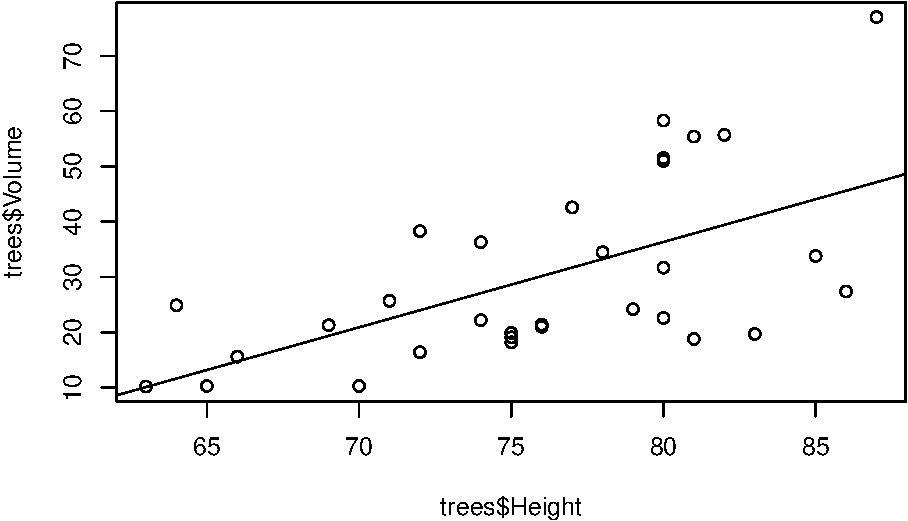
\includegraphics{Seminararbeit_files/figure-latex/unnamed-chunk-4-1.pdf}
\caption{Dataset and regression}
\end{figure}

By the way: the (\LaTeX) command \texttt{\textbackslash{}pagebreak} can
be used to force a page break.

\pagebreak

\hypertarget{citations}{%
\subsection{Citations}\label{citations}}

A \emph{bibtex} bibliography can be used for citations. The bibliography
file used in this template is \texttt{references.bib} and you find it in
the project directory. It is easily edited using \emph{RStudio}

A simple \emph{bibtex} entry looks like this:

\begin{verbatim}
@book{
  Hastie2013,
  publisher = {Springer},
  year = {2013},
  title = {The elements of statistical learning},
  author = {Hastie, Trevor and Tibshirani, Robert and Friedman, Jerome H.},
}
\end{verbatim}

The first field (\texttt{Hastie2013}) is the identifier which allows you
to cite a reference.

You can cite a source in Harvard style like this: \autocite{Hastie2013}
or \textcite{Hastie2013}.

A cited source will be automatically added to the reference section at
the end of the document.

\pagebreak

\hypertarget{conclusion}{%
\section{\texorpdfstring{Conclusion
\label{chap:conc}}{Conclusion }}\label{conclusion}}

Your conclusion. Note that you may also refer to a specific chapter or
section in the document, provided there is a label. We have anchored a
label to the section header of the Conclusion. You may reference it as
follow: See Chapter \ref{chap:conc}.

This section allows you to reference R packages used in the analysis.
Simply include them in \texttt{R\_packages.bib} as \emph{bibtex} entries
and include the identifiers using
\texttt{\textbackslash{}notecite\{...\}} as shown below.

\pagebreak

\addcontentsline{toc}{section}{References}
\printbibliography[title = References]
\cleardoublepage

\begin{refsection}
\nocite{R-base}
\nocite{R-Studio}

\printbibliography[title = Software-References]
\addcontentsline{toc}{section}{Software-References}
\end{refsection}

\cleardoublepage
\appendix
\setcounter{table}{0}
\setcounter{figure}{0}
\renewcommand{\thetable}{A\arabic{table}}
\renewcommand{\thefigure}{A\arabic{figure}}

\newgeometry{top=2.5cm, left = 2cm, right = 2cm, bottom = 2.5cm}

\hypertarget{appendix}{%
\section{Appendix}\label{appendix}}

\hypertarget{description-of-relevant-variables}{%
\subsection{\texorpdfstring{Description of relevant Variables
\label{app:A}}{Description of relevant Variables }}\label{description-of-relevant-variables}}

An example using the LaTeX environment \emph{longtable}:

\begin{longtable}{l|l|p{6cm}}
\caption{Description of relevant variables} \\
\hline
\textbf{Variable} & \textbf{Dataset} & \textbf{Description}    \\
\hline
\endfirsthead % Erster Kopf zu Ende
% Definition des Tabellenkopfes auf den folgenden Seiten
\caption{Description of relevant variables (continued)}\\
\hline
\textbf{Variable} & \textbf{Dataset} & \textbf{Description}    \\
\hline
\endhead % Zweiter Kopf ist zu Ende
\multicolumn{3}{r}{Continued on the next page.}\\
\endfoot
\hline
\multicolumn{3}{r}{End of table.} \\
\endlastfoot
Student.Pseudonym & all & Student’s immatriculation number \\
\hline
Semester & FS Data & Academic semester. The first four digits stand for the year, the fifth digit is either a 1 (summer semester) or a 2 (winter semester). Example: "20062" describes the winter semester 2006/2007, "20071" the summer semester 2007 \\
\hline
FS & FS, Pruefung Data & Study semester \\
\hline
Status & FS Data & Status as a student. "R" stands for re-enrollment, "N" for new enrollment, "E" for initial enrollment and "B" for leave of absence \\
\hline
Status.dpp & Pruefung Data & See variable Status \\
\hline
Austrittsgrund & FS, Studium Data & Reason for dropping out \\
\hline
SGCode & all & Code for study program. The last digit represents the examination regulations (PO). A change to the PO is thus considered as a new program in the system \\
\hline
Abschluss\_Bezeichnung & FS, Pruefung Data & Name of the degree that students receive upon successful completion of their studies \\
\hline
Fach\_Bezeichnung & FS, Pruefung Data & Name of the course of studies \\
\hline
PO & all & Examination regulations \\
\hline
PolyvalentePruefungsnummer & Pruefung Data & Polyvalent examination number \\
\hline
Bezeichnung & Pruefung Data & Name of the examination \\
\hline
Pruefungssemester & Pruefung Data & Semester in which the student was registered for the exam. Structure analogous to the variable ‘Semester’ in FS Data \\
\hline
Status.Pruefung & Pruefung Data & Status of the exam. "BE" means Passed, "ZU" means Withdrawn, "NB" means Not Passed and "PV" means Examination Existing (applications or performances are available, but the whole module is not yet completed) \\
\hline
Versuchszahl & Pruefung Data & Trial number \\
\hline
Note & Pruefung Data & Grade \\
\hline
VerbuchteECTSCP & Pruefung Data & Received ECTSCP \\
\hline
Start\_Semester & Studium Data & Semester in which the studies were started. Structure analogous to the variable ‘Semester’ in FS Data \\
\hline
Ende\_Semester & Studium Data & Semester in which the studies were finshed. Structure analogous to the variable ‘Semester’ in FS Data
\label{tab_var}
\end{longtable}

\end{document}